%----------------------------------------------------------------------------------------
%----------------------------------------------------------------------------------------
%----------------------------------------------------------------------------------------
%DATA
%----------------------------------------------------------------------------------------
%----------------------------------------------------------------------------------------
%----------------------------------------------------------------------------------------

\section{DATA}

%Our sample contains photometric and spectroscopic data of M31 and M101, as well as their measured properties such as SFR, stellar mass, dust luminosity, metallicity, and gas mass.    
For creating SOM, we used spectroscopy and photometry data as well as their measured properties such as SFR, stellar mass, dust luminosity and mass, metallicity, and gas mass from 10 regions in M31 (Fig~\ref{fig: regions in m31}) and 8 regions in M101 (Fig~\ref{fig: regions in m101}).
Table~\ref{tab: data} shows list of the sample and their unit for both M31 and M101.

\import{../sections/tables/}{tab_data.tex}

\begin{figure}
   \begin{subfigure}[b]{0.5\textwidth}
        \centering
    %\centering
        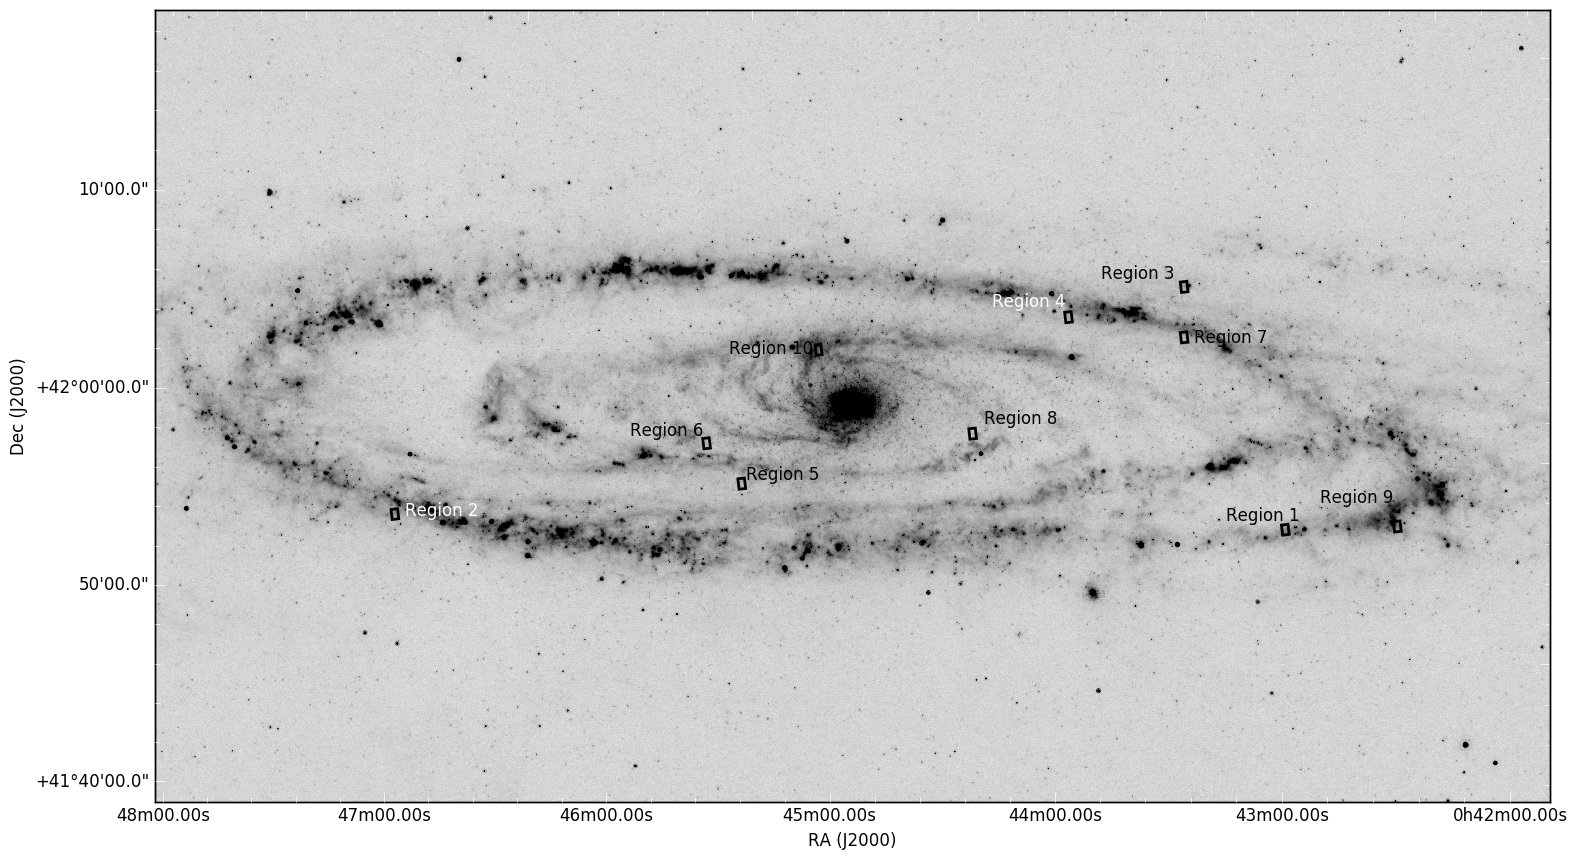
\includegraphics[width=0.97\textwidth]{../images/M31/M31_3.png}
        \caption{MIPS24 image of M31, with position of 10 regions that we studies.}
        \label{fig: regions in m31}
    \end{subfigure}
    \hfill
    \begin{subfigure}[b]{0.5\textwidth}
        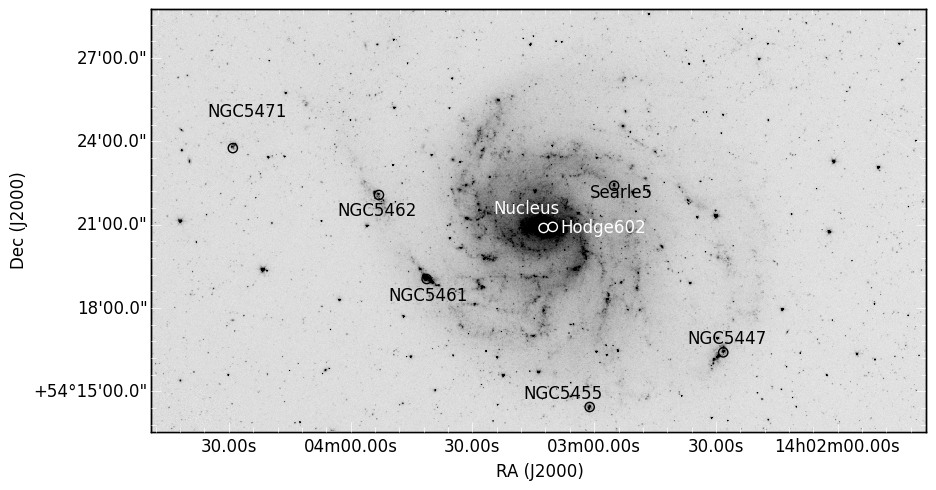
\includegraphics[width=\textwidth]{../images/M101/M101.png}
        \caption{IRAC1 image of M101, with position of our 8 regions that we studies.}
    \label{fig: regions in m101}
    \end{subfigure}
\end{figure}

%M31 data 
%%%%% Sahar: More detail?
    \subsection{M31 data}
      
     
     The 10 regions in M31 were chosen due to availability of the PAH data for them. 
     \cite{Dim15} studied PAH for those regions using {\it Spitzer}/Infrared Spectrograph\citep[IRS,][]{Houck04b} observations. 
     They used {\tiny PAHFIT IDL} tool~\citep{Smith07b} and measured fluxes and equivalent widths of PAH features as well as atomic line features.
     For spectroscopy part of our sample, we utilized their measured fluxes for PAH lines. 
     \cite{Dim15} also reported metallicity of these regions (using results from \cite{Sanders12} for most regions), which e used them in our input sample.
     We used radiation hardness index (RHI) instead of flux of individual atomic line, since they were only calculate the upper limit flux for most of the lines in most of the regions.
     
     For photometry part of the sample, we used data from \GALEX FUV and NUV channels~\citep{Martin05}, \halpha, [\sii] continuum and [\oiii] continuum emission~\citep{Massey07}, IRAC channels 1 to 4~\citep{Barmby06}, MIPS24 and 70~$\mu$m~\citep{Gordon06}, PACS100 and 160~$\mu$m and SPIRE250, 350, and 500~$\mu$m~\citep{Fritz12}.
     We changed units of all our data to Wm$^{-2}$ to be the same unit as PAH fluxes.
     We used $^{12}$CO (J:$1\rightarrow0$) line~\citep{Nieten06} and the atomic gas (H\,{\sc I}) 21~cm emission from \cite{Chemin09}.
     We also utilized SFR(FUV + 24$\mu$m), stellar mass, total gas mass, and total infrared (TIR) emission data from \cite{Rahmani16}, and dust luminosity and mass data from \cite{Draine14}.


%M101 data: observed ones;
    \subsection{M101 data}
     For M101 galaxy, we used PAH fluxes which had been measured using {\tiny PAHFIT IDL} tool and reported in \cite{Gordon08}.
     We also added their measurement of metallicity and RHI for these regions to our sample.
     We used data available on NED~\footnote{The NASA/IPAC Extragalactic Database (NED) is operated by the Jet Propulsion Laboratory, California Institute of Technology, under contract with the National Aeronautics and Space Administration.} website to gather our photometry data of M101. 
     We chose data from \GALEX FUV and NUV channels~\citep{depaz07}, IRAC channels 1 to 4, MIPS~24 and 70~$\mu$m~\cite{Dale09}, and  PACS~100 and 160~$\mu$m and SPIRE250, 350, and 500~$\mu$m~\cite{Kennicutt11}.
     Same as M31 data, we used $^{12}$CO (J:$1\rightarrow0$) line~\citep{Helfer03} and the atomic gas (H\,{\sc I}) 21~cm emission from \cite{Walter08} data.
     SFR(FUV + 24$\mu$m), stellar and total gas map were calculated followed method described in \cite{Rahmani16} to create these maps.
     